	\documentclass[11pt,a5paper]{article}
\usepackage[utf8]{inputenc}
\usepackage[english]{babel}
\usepackage{amsmath}
\usepackage{amsthm}
\usepackage{amsfonts}
\usepackage[margin=0.47in]{geometry}
\usepackage{graphicx}

\newtheorem{theorem}{Example}
\newtheorem{exercise}{Exercise}
\newtheorem*{Theorem}{Theorem}

\title{\textbf{Geometry I.}}
\date{Week 8}
\author{Miroslav Stankovic\\ Marko Puza}
\begin{document}
\maketitle

\section{Theory}

\noindent One of the most beautiful (I might be biased here) topics in problem solving is Euclidean geometry. To solve a geometric problem you often need to have a cunning perspective over the whole problem and employ creativity. \\
In this sheet we will briefly iterate over some well-known theorems and look in more detail into properties of cyclic quadrilaterals. \\
Let us adapt the notation $\alpha = \beta$, which denotes that angles $\alpha, \beta$ are \emph{congruent} (equal in measure).
\subsection*{Basic theorems}

\begin{Theorem}[Parallel lines]
	In the figure below, the lines $x$ and $y$ are parallel. Then we have  $a=c=g=e$, $b=d=f=h$, and $b+g = 180^{\circ}$.
\end{Theorem}

\begin{figure}[h] \begin{center}
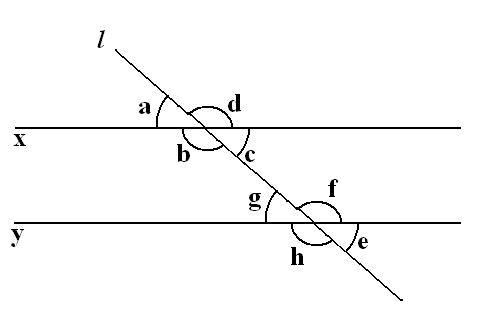
\includegraphics[width=0.5\textwidth]{parallel}
\end{center} \end{figure}
\noindent Pair of angles $a, e$ is an example of \emph{alternate exterior angles}.\\
\noindent Pair of angles $c, g$ is an example of \emph{alternate interior angles}.\\
\noindent Pair of angles $a, c$ is an example of \emph{vertical angles}.
\begin{exercise}
In the figure 1, supposte that $a=3x-33^{\circ}$ and $h=7x+3^{\circ}$. Find $x$.
\end{exercise}

\begin{Theorem}[Similarity of triangles]
Two triangles are similar if and only if corresponding angles are congruent and the lengths of corresponding sides are proportional. \\
Furthermore, two triangles are similar if:
\begin{itemize}
\item{\textbf{aa}: the triangles have two congruent angles}
\item{\textbf{sss}: all corresponding sides have lengths in the same ratio}
\item{\textbf{sas}: two sides have lengths in the same ratio, and the angles included between these sides are congruent}
\end{itemize}
\end{Theorem}

\begin{exercise}
Prove $aa$, $sss$ and $sas$ conditions above.
\end{exercise}


\begin{Theorem}[Pythagoras theorem]
	In arbitrary right-angled triangle (figure below) \[|AB|^2 + |AD|^2 = |BD|^2\]
\end{Theorem}
\begin{Theorem}[Thales' theorem]
	$BD$ is diameter of circumcircle of $\triangle ABD$.
\end{Theorem}
\begin{Theorem}[Geometric mean theorem]
	\ \\Altitude Rule: $|CA|^2 = |CD| \cdot |CB|$.\\
	Leg Rule: \ \ \ \ \ \  $|BA|^2 = |BC| \cdot |BD|$.
\end{Theorem}

\begin{center}
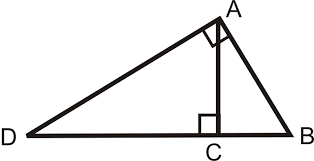
\includegraphics[width=0.5\textwidth]{right}
\end{center}

\begin{exercise} Prove \emph{Geometric mean theorem} (both rules).
\end{exercise}
\break
\begin{Theorem}[Central angle theorem]
Let $AB$ be arbitrary arc of a circle with center $O$ and $C$ arbitrary point lying on a circle, but not on arc $AB$. Then \[\angle AOB = 2\angle ACB\]
\end{Theorem}
\begin{proof}
We will prove the case when $O$ lies between segments $BC$ and $AC$. \\
Denote $\angle ACO$ as $x$ and $\angle BCO$ as $y$. Since $\triangle AOC$ is isosceles triangle, $\angle CAO = x$ and $\angle AOC = 180^\circ - 2x$. Analogically, $\angle BOC = 180^\circ - 2y$. \\ Since angles $\angle AOC$, $\angle BOC$ and $\angle AOB$ must add up to $360^\circ$, we must have $\angle AOB = 2x + 2y$. \\
In the figure above, $\alpha = 2x + 2y = 2(x + y) = 2\theta$.
\end{proof}

\begin{center}
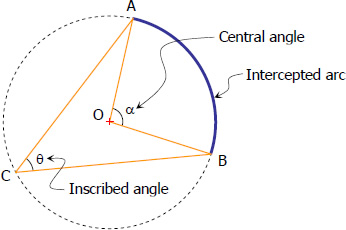
\includegraphics[width=0.5\textwidth]{central}
\end{center}

\begin{exercise}
Prove the general case of Central angle theorem.
\end{exercise}

\begin{Theorem}[Circumscribed angles]
Let $AB$ be arc of a circle centered in $O$ (such that length of this arc spans at most half of the circle) with corresponding inscibed angle $\alpha$. Then the angles between the tangent lines to a circle in points $A, B$ and the line segment $AB$ is congruent to $\alpha$.
\end{Theorem}
\begin{proof}
Since $\triangle AOB$ is isosceles and by the central angle theorem $\angle AOB = 2\alpha$, we must have $\angle OAB = \angle OBA = 90^\circ - \alpha$.
Combining this with the fact that segment $OA$ is perpendicular to the tangent line at point $A$, we obtain the sought result. 
\end{proof}

\begin{center}
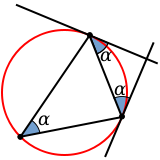
\includegraphics[width=0.3\textwidth]{circum}
\end{center}

\subsection*{Cyclic quadrilaterals}
\textbf{Many} geometric problems are solvable only by seeking cyclic quadrilaterals in them and applying their properties. Let us take a good look at them:
\begin{center}
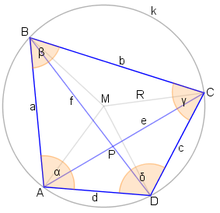
\includegraphics[width=0.38\textwidth]{cyclic}
\end{center}

\begin{Theorem}[Properties of cyclic quadrilaterals]
The following statements are all equivalent:\\
- ABCD is cyclic quadrilateral\\
- Points $A,B,C,D$ all lie on a common circle \\
- Each exterior angle of $ABCD$ is equal to the opposite interior angle.\\
- The four perpendicular bisectors to the sides are concurrent. Their common point of intersection is the circumcenter. \\
- Angle between any side and one diagonal is equal to the angle between opposite side and the other diagonal. That is, for instance,  $\angle ABD = \angle ACD$ \\
- The opposite angles are supplementary\footnote{they add up to $180^\circ$}, that is: $\alpha + \gamma = \beta + \delta = 180^\circ$\\
\end{Theorem}

\begin{exercise}
Try to find the reasons for why the above properties hold, using central angle theorem.
\end{exercise}

\noindent We will conclude the theory section by looking at two more interesting properties of cyclic quadrilaterals:

\begin{Theorem}[Ptolemy's theorem] 
Let $e,f$ denote the lenghts of diagonals of a cyclic quadrilateral $ABCD$ with lengths of the sides $a,b,c,d$. Then \[ef = ac + bd\]
\end{Theorem}

\begin{Theorem}[Brahmagupta's formula]
The area $A$ of a cyclic quadrilateral can be found as \[A = \sqrt{(s-a)(s-b)(s-c)(s-d)}\]
where $s = \frac{a+b+c+d}{2}$ is the semiperimeter.
\end{Theorem}

\section{Problems}


\begin{enumerate}
	\subsection*{Easy}

\item{Let $ABCD$ be a parallelogram, $W, X, Y, Z$ points on the sides \\ $AB, BC, CD, DA$ and $S$ intersection of $XZ$ with $WY$. $AWSZ$ is cyclic. Prove that also $BXSW, XCYS, YDZS$ are cyclic.}

	\item{We are given triangle $ABC$. Angle bisector of $\angle BCA$} intersect circumcircle of $\triangle ABC$ in point \v{S}. Prove that \v{S} is midpoint of arc $AB$.
	
	\item{Circles $l$ and $k$ intersect in points $A$, $B$. Choose point $X$ on the circle $k$ and let $Y$ be intersection of $l$ with line $XB$. Show that $\angle AXY$ does not depend on choice of $X$}

	\subsection*{Medium}
	
	\item{Given triangle $ABC$, let $H$ be intersection of its altitudes (orthocenter). Prove that reflection of $H$ over line $AB$ lies on the circumcircle of $\triangle ABC$}	
	
	\item{Let the points of intersection of the altitudes with the sides of the triangle $\triangle ABC$ be $D$, $E$, and $F$. Show that altitudes of $\triangle ABC$ are angle bisectors in $\triangle DEF$.}
	
	\item{Let $ABC$ be a triangle with right angle at $C$ and $M$ be a point on line segment $AB$. Let $S$, $S_1$, and $S_2$ be circumcentres of triangles $ABC$, $ AMC$, $BMC$ Show that $M$, $C$, $S$, $S_1$, and $S_2$ lie on a circle. }
		
	\item{Given triangle $ABC$ and a point $D$ on its circumcircle, let $P$, $Q$, $R$ be points closest to $D$ on sides $AB$, $BC$, $CA$. Prove that $P$, $Q$, $R$ colinear.}
	
	
	
\subsection*{Difficult}
	
	\item{Points $A, B, C, D, E, F$ lie on a circle. Let $AE$ and $BF$ intersect at $P$, $BD$ and $CE$ at $R$, and $AD$ and $CF$ at $S$. Show that $P$, $R$, $S$ are colinear.}
	
	\item{Let $O$ be circumcenter of triangle $ABC$. Line through $O$ intersect sides $AB$ and $AC$ in $M$ and $N$. Let $R$, $S$ be midpoints of $CM$, $BN$. Show that $\angle ROS = \angle BAC$}

\end{enumerate}

\begin{thebibliography}{9}
\bibitem{KMS} Ondrej Budáč, Tomáš Jurík, and Ján Mazák. 
	\emph{Zbierka úloh KMS}. Trojsten, Bratislava, 2010.
	
\bibitem{PraSe} Matematický korespondenční seminář. Knihovna. [ONLINE] Available at: \texttt{https://mks.mff.cuni.cz/library/library.php}. [Accessed November 10].
\end{thebibliography}
\end{document}
